% !TEX TS-program = pdflatexmk
\documentclass{beamer}
 
\usepackage[utf8]{inputenc}
\setbeamertemplate{bibliography item}{\insertbiblabel}
\usetheme{Madrid}
\usecolortheme{default}
\usepackage{caption}
\usepackage{subcaption}
\usepackage{hhline}
\usepackage{graphicx}
\usepackage{physics}
\usepackage{amsmath}
\usepackage{amsfonts}
\usepackage{esint}
\usepackage{bbold}
\usepackage{mathtools}
\usepackage{dsfont}
\usepackage{amsthm}
\usepackage{bbm}
\usepackage{amssymb}
\theoremstyle{definition}
\newtheorem{defn}{Definition}[section]
\newtheorem{prop}{Properties}[section]
\newtheorem{rmk}{Remark}[section]
\newtheorem{exmp}{Example}[section]
\newtheorem{prob}{Problem}[section]
\newtheorem{proposition}{Proposition}
\newtheorem{thm}{Theorem}[section]
\newtheorem*{prob*}{Problem}
\newtheorem*{sln*}{Solution}
\usepackage{empheq}
\usepackage{tensor}
\usepackage{MnSymbol,wasysym}

\newcommand{\lag}{\mathcal{L}}
\newcommand{\pOne}{\text{5p}_\text{1/2}}
\newcommand{\pThree}{\text{5p}_\text{3/2}}
\newcommand{\potassium}{^\text{39}\text{K}}
\newcommand{\R}{\mathbb{R}}
\newcommand{\lp}{\left(}
\newcommand{\rp}{\right)}
\newcommand{\lb}{\left[}
\newcommand{\rb}{\right]}
\newcommand{\lc}{\left\{}
\newcommand{\rc}{\right\}}
\newcommand{\p}{\partial}
\newcommand{\f}[2]{\frac{#1}{#2}}
\newcommand{\Vol}{\operatorname{Vol}}
\newcommand{\iprod}{\mathbin{\lrcorner}}
\newcommand{\al}{\alpha}
\newcommand{\be}{\beta}
\newcommand{\FT}{\mathcal{F}}
\newcommand{\LT}{\mathcal{L}}
\usepackage{hyperref}
\usepackage{tensor}
\usepackage{xcolor}
\hypersetup{
	colorlinks,
	linkcolor={black!50!black},
	citecolor={blue!50!black},
	urlcolor={blue!80!black}
}

% 3j symbol
\newcommand{\tj}[6]{ \begin{pmatrix}
		#1 & #2 & #3 \\
		#4 & #5 & #6 
\end{pmatrix}}
% 6j symbol
\newcommand{\Gj}[6]{ \begin{Bmatrix}
		#1 & #2 & #3 \\
		#4 & #5 & #6 
\end{Bmatrix}}

\setbeamerfont{title}{size=\large}

 
 
%Information to be included in the title page:
\title[\textcolor{white}{{}}]
{
The Hydrogen Atom and Harmonic Oscillator(s)
}



\author[Bui] % (optional)
{Huan Bui}
\institute[MIT]{MIT} % (optional)
\date{ZGS, Mar 24, 2023}
  
\begin{document}
 
\frame{\titlepage}

\begin{frame}
	\frametitle{Harmonic oscillator universe?}
	
	\begin{minipage}{0.39\textwidth}
	\begin{figure}
	\centering
	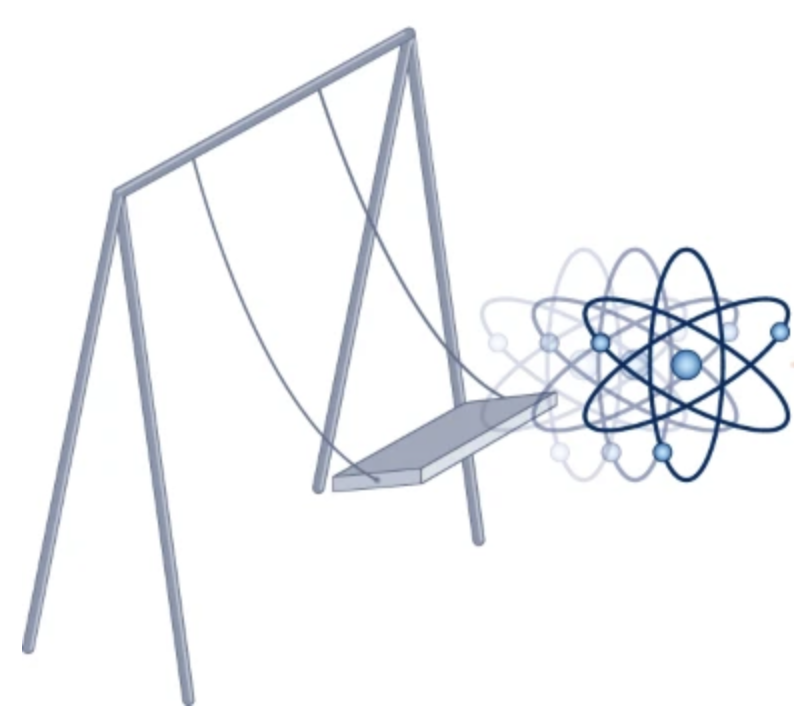
\includegraphics[width=1\textwidth]{figures/swinging_atom.png}
	\end{figure}
	\end{minipage}
	\begin{minipage}{0.6\textwidth}
	Harmonic oscillator in physics: 
	\begin{itemize}
		\item Hooke's law 
		\item QHO 
		\item Einstein solid 
		\item Atom-radiation interaction 
		\item 2nd quantization of EM fields  
		\item QFT 
		\item $\dots$ \pause
		\item \textcolor{purple}{Gravity? Inverse-square law?}	
	\end{itemize}
	\end{minipage}
	
	
	
\end{frame}


\begin{frame}
	\frametitle{Coulomb-Kepler problem revisited}
	A particle in a central potential $V(r) = -k/r$:
	\begin{align*}
	H = \f{\vec{p}^2}{2m} - \f{k}{r}.
	\end{align*}
	
	\pause
	
	Constants of motion: $H$, \pause
	$\vec{L} = \vec{r}\times \vec{p}$,  \pause
	and $\vec{A}$, \pause
	the \textcolor{purple}{Laplace-Runge-Lenz} vector:
	\begin{align*}
	\vec{A} = \vec{p}\times \vec{L} - m k \f{ \vec{r}}{r}.
	\end{align*}	
	
	
	\end{frame}



\begin{frame}
\frametitle{Coulomb-Kepler problem revisited}

Brief review: 
\begin{figure}
\centering
\includegraphics[width=0.6\textwidth]{figures/LRL.eps}
\end{figure}

\pause

$\vec{A}$ is in the plane of the orbit (so $\vec{A}\cdot \vec{L} = 0$), with ${A}^2 = m^2 k^2 + 2m E {L}^2$. \\
\,\,\, \\  \pause
$\vec{A}$ determines the shape and orientation of the orbit.


\end{frame}


\begin{frame}
\frametitle{Coulomb-Kepler problem revisited}
$\vec{A}$ determines the shape and orientation of the orbit: \pause

\begin{itemize}

\item Shape: from
\begin{align*}
\vec{A} \cdot \vec{r} = \vec{r} \cdot (\vec{p} \times \vec{L}) - m k = (\vec{r}\times \vec{p})\cdot \vec{L} - m k = L^2 - m k  =  A r \cos\theta
\end{align*}
\pause
we get the orbit equation
\begin{align*}
\f{1}{r} = \f{m k }{L^2} \lp 1 + \epsilon \cos\theta \rp, \quad  
\text{eccentricity } \epsilon = \f{A}{\abs{ m  k}} = \sqrt{1 + \f{2EL^2}{m k^2}} \geq 0
\end{align*}\pause 

\item Orientation: $\vec{A}$ points from source to periapsis
\end{itemize}

\end{frame}


\begin{frame}
\frametitle{Aside: Brief history of the LRL vector}


\pause

Unclear origin, gets rediscovered repeatedly:\pause
\begin{itemize}
	\item Neither Laplace, Runge, nor Lenz discovered it. Laplace (1799) \pause
	\item Jakob Hermann discovered $|\vec{A}|$ (1710), recognized its relation to $\epsilon$ \pause
	\item  Johann Bernoulli generalized to $\vec{A}$ (1710) \pause
	\item Hamilton "rediscovered" $\vec{A}$ as $\vec{A}/m k$ ($\sim$1850) \pause
\end{itemize}
\,\,\, \\ 
Pauli and the LRL vector in early QM (1926): \pause
\begin{itemize}
	\item Used $\vec{A}$ to derive the spectrum of hydrogen (pre-SE!) \pause
	
	\item Derived energy shifts in the presence of $\vec{E}$ and $\vec{B}$ \pause
\end{itemize}

\pause

\,\,\, \\
Further readings (so fun):  

\begin{itemize}
\item History: \cite{valent2003hydrogen}, 
\cite{stahlhofen2004pauli},
\cite{goldstein1975prehistory},
\cite{goldstein1976more},
\cite{goldstein2002classical}


\item "Discoveries"  and application: 
\cite{runge1919vektoranalysis},
\cite{laplace1823traite},
\cite{lenz1924bewegungsverlauf},
\cite{hamilton1847application},
\cite{hermann1710unknown},
\cite{pauli1926wasserstoffspektrum}
\end{itemize}

\end{frame}




\begin{frame}
	\frametitle{The Hydrogen Atom}
	
	The energy levels and wavefunctions for the bound states of hydrogen are gotten by solving the Schr\"{o}dinger equation:
	
	\begin{align*}
	\lc -\f{\hbar^2 }{2m} \nabla^2 - \f{e^2}{r} \rc \psi = E\psi, \quad\quad E < 0.
	\end{align*}
	
	\pause
	
	With
	\begin{equation}
	\label{eq:conds}
	\lambda = \f{8}{a} \quad\quad \al^4 = -\f{8E}{e^2 a}, \quad\quad a = \f{\hbar^2}{m e^2},
	\end{equation}
	the SE becomes
	\begin{equation}\label{eq:SE}
	\lc 4\nabla^2 + \f{\lambda}{r} -\al^4  \rc \psi = 0.
	\end{equation}
	
\end{frame}


\begin{frame}
	\frametitle{Where are the harmonic oscillators? }
	
	Following \cite{cornish1984hydrogen}, introduce coordinates $\zeta_A, \zeta_B \in \mathbb{C}$ and demand
	\begin{align*}
	x + iy = 2 \zeta_A  \overline{\zeta_B} 
	\quad\quad\quad\quad\quad   
	z = \zeta_A \overline{\zeta_A}  -  \zeta_B \overline{\zeta_B}  .
	\end{align*}
	\pause
	With this,
	\begin{align*}
	r = \sqrt{x^2 + y^2 + z^2} = \zeta_A \overline{\zeta_A}  +  \zeta_B \overline{\zeta_B} 
	\end{align*}
	
	Note:
	\begin{itemize}
	\item Each pair $(\zeta_A, \zeta_B)$ gives a unique point $(x,y,z)$
	
	\item Converse is true up to arbitrary but equal arguments of $\zeta_A, \zeta_B$
	\end{itemize}
	
\end{frame}


\begin{frame}
	\frametitle{Where are the harmonic oscillators? }
	
	Let $\sigma = 2\arg(\zeta_A) = 2\arg(\zeta_B)$. Can write $\zeta_A, \zeta_B$ in spherical coordinates:
	\begin{equation}\label{eq:coords}
	\zeta_A = r^{1/2} e^{i (\sigma + \varphi)/2}   \cos  \f{\theta}{2}  
	\quad\quad 
	\zeta_B = r^{1/2} e^{i(\sigma - \varphi)/2}  \sin \f{\theta}{2} 
	\end{equation}
	$\implies$ $(x,y,z)$ determines $(\zeta_A, \zeta_B)$ up to $e^{i\sigma}$.
	
	
	\vspace{15pt}
	\pause
	
	Can show that
	\begin{align*}
	r \nabla^2 \psi = (\p_A \p_{\bar{A}} + \p_B \p_{\bar{B}}) \psi.
	\end{align*}
	$\implies$ Can now write SE in terms of $\zeta_A, \zeta_B, \overline{\zeta_A}, \overline{\zeta_B}$. 
	
	

\end{frame}


\begin{frame}
	\frametitle{Where are the harmonic oscillators?}
	SE in terms of $\zeta_A, \zeta_B, \overline{\zeta_A}, \overline{\zeta_B}$:
	\begin{equation}
	\label{eq:zeta1}
	\lc 4\nabla^2 + \f{\lambda}{r} -\al^4  \rc \psi 
	= 
	\lc 4 (\p_A \p_{\bar{A}} + \p_B \p_{\bar{B}}) + \lambda - \al^4 (\zeta_A \overline{\zeta_A} + \zeta_B \overline{\zeta_B}) \rc \psi = 0
	\end{equation}
\pause	
	Since $\psi(x,y,z)$ independent of $\sigma$,
	\begin{equation}\label{eq:zeta2}
	\f{\p \psi}{\p \sigma} = 0 \quad \iff \quad 
	(\overline{\zeta}_A \p_{\bar{A}} - \zeta_A \p_{A})\psi =
	-(\overline{\zeta}_B \p_{\bar{B}} - \zeta_B \p_{B})\psi.
	\end{equation}
	\pause
	Together, \eqref{eq:zeta1} and $\eqref{eq:zeta2}$ are equivalent to SE \eqref{eq:SE}. 
\end{frame}



\begin{frame}
	\frametitle{Where are the harmonic oscillators?}
	
	Let $\zeta_A = q_1 + iq_2$ and $\zeta_B = q_3 + iq_4$, then \eqref{eq:zeta1} is the equation for a 4D HO
	\begin{equation}\label{eq:4d-sho}
	[\p_1^2 + \p_2^2 + \p_3^2 + \p_4^2 + \lambda - \al^4(q_1^2 + q_2^2 + q_3^2 + q_4^2)] \psi = 0
	\end{equation}
	\pause
	with frequency $\omega$ and energy $\epsilon$ given by \eqref{eq:conds}:
	\begin{align*}
	\al^2 \equiv \sqrt{-\f{8E}{e^2 a}} = \f{m \omega}{\hbar} 
	\quad\quad\quad 
	\lambda \equiv \f{8}{a} = \f{2m \epsilon}{\hbar^2}.
	\end{align*}
	
	\pause 
	Condition \eqref{eq:zeta2} becomes
	\begin{equation}
	\label{eq:ang}
	(q_1 \p_2 - q_2 \p_1) \psi = -(q_3 \p_4 - q_4 \p_3)\psi.
	\end{equation}
	
	\eqref{eq:4d-sho}$ + \eqref{eq:ang}:$ 
	\textcolor{purple}{Two 2D HO's with equal and opposite angular momenta}
\end{frame}




\begin{frame}
	\frametitle{From harmonic oscillators to hydrogen}
	
	Separating variables $\psi = \psi(q_1, q_2) \psi(q_3, q_4)$, 
	\begin{align*}
	&[\p_1^2 + \p_2^2 + \lambda_A - \al^4(q_1^2 + q_2^2)]\psi_A = 0,
	\end{align*}
	with $\lambda_A = 2 m \epsilon_A / \hbar^2$.  \pause Solution for $A$: 
	\begin{align*}
	&\psi_{A n_A m_A}  = C_{n_Am_A} \lp \f{\zeta_A }{\overline{\zeta_A}} \rp^{{m_A}/2}  
	\lp\al^2 \zeta_A \overline{\zeta_A}\rp^{\abs{m_A}/2}e^{ -\f{\al^2 \zeta_A \overline{\zeta_A}}{2} } 
	L_{n_A + \abs{m_A}}^{\abs{m_A}} \lp \al^2 \zeta_A \overline{\zeta_A} \rp\\
	&\quad n_A = 0,1,2,\dots \quad 
	m_A = 0, \pm 1, \pm 2, \dots  \\ 
	%L_{n_A + \abs{m_A}}^{\abs{m_A}}: \text{ assoc. Laguerre polys}\\
	&\text{\textcolor{purple}{Energy: }} \epsilon_{A n_A m_A} = \hbar \omega(2n_A + \abs{m_A} + 1) = \f{\hbar^2 \lambda_{An_A m_A}}{2m}\\
	&\text{\textcolor{purple}{Angular momentum: }} L_{A n_A m_A} = m_A \hbar 
	\end{align*}
	Similar solution for $B$. $\lambda_A + \lambda_B = \lambda$ and $m_A = -m_B = m$ due to \eqref{eq:ang}.
\end{frame}



\begin{frame}
\frametitle{From harmonic oscillators to hydrogen}

Full solution
\begin{align*}
\psi_{n_A n_B m} = \psi_{An_A m}\lp \zeta_A, \overline{\zeta_A}\rp \psi_{Bn_B- m}\lp \zeta_B, \overline{\zeta_B} \rp.
\end{align*}

\pause 

Can relate this back to the hydrogen atom. \pause From 
\begin{align*}
\lambda = \lambda_A + \lambda_B =  4\al^2 (n_A + n_B + \abs{m} + 1) = \f{8}{a}
\end{align*}
can get energy in terms of $n_A, n_B, m$:
\begin{align*}
E = \f{-\al^4 e^2 a}{8} = -\f{\al^4 e^2 }{\lambda} = \f{-e^2 }{2a(n_A + n_B + \abs{m} + 1)^2} \equiv \f{-e^2}{2aN^2}.
\end{align*}


\end{frame}



\begin{frame}
\frametitle{From harmonic oscillators to hydrogen}
How about the wavefunctions? 
\pause Going to parabolic coordinates $(\xi, \eta, \varphi)$:
\begin{align*}
&x = \sqrt{\xi\eta}\cos\varphi \quad\quad y = \sqrt{\xi\eta}\sin\varphi \quad\quad z = (\xi - \eta)/2\\
\iff 
&\xi = 2r\cos^2 (\theta/2) = 2\abs{\zeta_A}^2  \quad\quad \eta = 2r\sin^2 (\theta/2) = 2\abs{\zeta_B}^2. 
\end{align*}
\pause
we get
\begin{align*}
\psi_{n_A n_B m} = K_{n_An_B m} e^{im\varphi} (\xi \eta)^{\abs{m}/2}  e^{ -\f{\al^2(\xi^2 + \eta^2)}{4}}
L_{n_A + \abs{m}}^{\abs{m}} \lp\f{\al^2 \xi}{2} \rp
L_{n_B + \abs{m}}^{\abs{m}} \lp\f{\al^2 \eta}{2} \rp.
\end{align*}
\pause 
These are simultaneous eigenfunctions of $\mathbf{H}$, 
\pause $\mathbf{L}_z$, 
\pause and $\mathbf{M}_z$ where
\begin{align*}
\mathbf{M} = \f{1}{2m} (\mathbf{p}\times \mathbf{L} - \mathbf{L}\times \mathbf{p}) - \f{e^2}{r} \mathbf{r}.
\end{align*}
is the \textcolor{purple}{Laplace-Runge-Lenz operator}, symmetrized by Pauli, 1926.

\end{frame}




\begin{frame}
\frametitle{From harmonic oscillators to hydrogen}
From how $(\zeta_A, \zeta_B)$ is defined:
\begin{align*}
\mathbf{M}_z = \f{e^2a}{r} 
\lb  
\abs{\zeta_B}^2 \p_A \p_{\bar{A}}  
- \abs{\zeta_A}^2 \p_B \p_{\bar{B}} 
-  \f{1}{a} ( \abs{\zeta_A}^2 + \abs{\zeta_B}^2) 
\rb.
\end{align*} 
\pause 
CSCO is $\{ \mathbf{H}, \mathbf{L}_z, \mathbf{M}_z \}$ instead of $\{ \mathbf{H}, \mathbf{L}^2 , \mathbf{L}_z \}$. Eigenvalue equations:
\begin{align*}
\mathbf{H} \psi_{n_A n_B m} &= \f{-e^2}{2aN^2} \psi_{n_A n_B m} \\
\mathbf{L}_z \psi_{n_A n_B m} &= m \hbar \psi_{n_A n_B m}\\
\mathbf{M}_z \psi_{n_A n_B m} &= \f{e^2 (n_B - n_A)}{N}  \psi_{n_A n_B m}.
\end{align*}
\pause
\vspace{-10pt}
\begin{align*}
[\mathbf{M}_z, \mathbf{L}^2] \neq 0, 
\quad\quad 
[\mathbf{M}_z, \mathbf{M}^2] \neq 0, 
\quad\quad 
[\mathbf{M}^2, \mathbf{H}] = [\mathbf{M}^2, \mathbf{L}^2] = [\mathbf{M}^2, \mathbf{L}_z] = 0.
\end{align*}
\end{frame}



\begin{frame}
\frametitle{Aside: Hydrogen wavefunctions in parabolic coordinates}

What do eigenfunctions of $\mathbf{M}_z$ look like? 
\begin{align*}
\psi_{n_A n_B m} = K_{n_An_B m} e^{im\varphi} (\xi \eta)^{\abs{m}/2}  e^{ -\f{\al^2(\xi^2 + \eta^2)}{4}}
L_{n_A + \abs{m}}^{\abs{m}} \lp\f{\al^2 \xi}{2} \rp
L_{n_B + \abs{m}}^{\abs{m}} \lp\f{\al^2 \eta}{2} \rp.
\end{align*}

\pause

\begin{figure}[!htb]
\begin{minipage}{0.24\textwidth}
\includegraphics[width=0.95\textwidth]{figures/000.eps}
\caption*{$(0,0,0)$}
\end{minipage}
\begin{minipage}{0.24\textwidth}
\includegraphics[width=0.95\textwidth]{figures/200.eps}
\caption*{$(2,0,0)$}
\end{minipage}
\begin{minipage}{0.24\textwidth}
\includegraphics[width=0.95\textwidth]{figures/212.eps}
\caption*{$(2,1,2)$}
\end{minipage}
\begin{minipage}{0.24\textwidth}
\includegraphics[width=0.95\textwidth]{figures/413.eps}
\caption*{$(4,1,3)$}
\end{minipage}
\caption{$\abs{\psi_{n_An_Bm}(x,0,z)}^2$ for different values of  $(n_A, n_B, m)$ \cite{blinder2011}}
\end{figure}

\end{frame}


\begin{frame}
\frametitle{Shouldn't the correspondence be classical?}


Following \cite{chen1987coulomb}, use the Kustaanheimo-Stiefel transformation $S: \mathbb{R}^4\to \mathbb{R}^3$:
\begin{align*}
x_1 &= 2(s_1s_3 - s_2s_4) \\
x_2 &= 2(s_1s_4+s_2s_3) \\ 
x_3 &= s_1^2 + s_2^2 - s_3^2 - s_4^2
\end{align*}

\pause 

Only three of $\{ s_1,s_2,s_3,s_4 \}$ are independent. What is the constraint? \pause
\begin{align*}
\begin{cases*}
x_1 = r \sin\theta\cos \phi \\ 
x_2 = r \sin\theta\sin \phi \\ 
x_3 = r\cos\theta
\end{cases*}
\quad\quad\quad 
\begin{cases*}
s_1 = s\cos\alpha \cos\beta \\ 
s_2 = s\cos\alpha \sin\beta \\
s_3 = s\sin\alpha \cos\gamma \\ 
s_4 = s\sin\alpha \sin\gamma
\end{cases*}
\end{align*}

\pause 
Constraint on coordinates: $r = s^2,\quad  \theta = 2 \alpha, \quad \phi = \be + \gamma$

\pause 
Constraint on velocities: $s_2\dot{s}_1 - s_1 \dot{s}_2 - s_4 \dot{s}_3 + s_3 \dot{s}_4 = 0$

\end{frame}



\begin{frame}
\frametitle{Shouldn't the correspondence be classical?}

\underline{The equivalence}: With $4\abs{E} = m\omega^2/2 $ and $\epsilon = 4k$,
\begin{align*}
\f{1}{2} mv^2  - \f{k}{r} = -\abs{E} 
\quad \xrightarrow{\quad} \quad
\f{1}{2} m \dot{s}^2 + \f{1}{2} m\omega^2 s^2 = \epsilon \quad \text{(4D H.O.)}
\end{align*}
\,\,\,
\pause 
In polar coordinates: \pause $u = s \cos\alpha, v = s\sin\alpha$
\begin{align*}
\f{1}{2}m (\dot{u}^2 + u^2 \dot{\beta}^2 + \dot{v}^2 + v^2 \dot{\gamma}^2 ) + \f{1}{2} m\omega^2 (u^2 + v^2) = \epsilon.
\end{align*}
\pause 
The constraint on velocities $\iff \vec{L} \cdot \vec{M} = 0$ \pause and implies
\begin{align*}
 -u^2 \dot{\be} + v^2 \dot{\gamma} = 0 \implies  
 mu^2\dot{\be} = m v^2 \dot{\gamma} 
 \implies   L_\be = L_\gamma
\end{align*}
\pause 
$\implies$ \textcolor{purple}{Two coupled 2D H.O.'s with equal angular momenta}
\end{frame}


\begin{frame}
\frametitle{Something deeper?}

Symmetry implies degeneracy. $[\mathbf{M}, \mathbf{H}] = 0 $ explains the $n^2$ degeneracy in $H$. 

\begin{figure}[!htb]
\centering
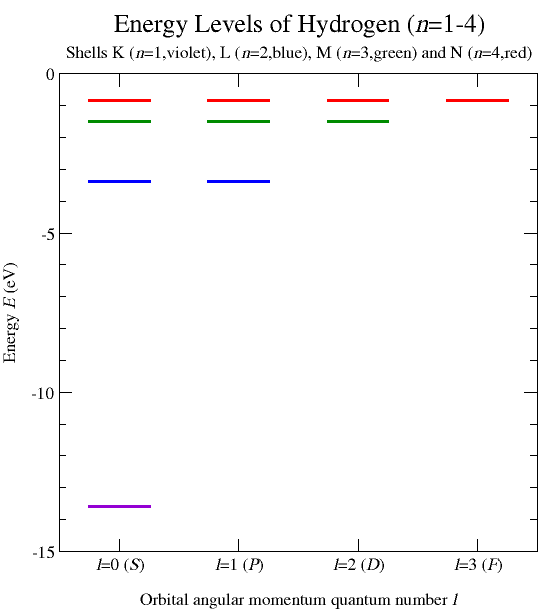
\includegraphics[width=0.4\textwidth]{figures/Hydrogen_energy_levels.png}
\end{figure}

More info: SO(4) symmetry of H, etc. See Chapter 14 of \cite{gilmore2008lie}. 

\end{frame}





\begin{frame}[allowframebreaks]
	\frametitle{References}
	\fontsize{6pt}{7pt}\selectfont
	
 	\bibliographystyle{unsrt}
	\bibliography{references.bib}
\end{frame}








\end{document}